\chapter{Related work}
\label{chap:related}

In this chapter we provide overview of the methods used for detections in video. There are two categories of detectors that can be used for video detection, a very fast single frame detectors, or a detector designed for a sequence of frames. Although there is no definition of what is real time, generally 25fps is considered as the lower bound. However in practise we need as much fps as possible to process multiple video streams. 

\section{Real-time detectors}

\subsection{YOLO: You Only Look Once (2016)}
\label{sec:yolo}
Building on the success of neural network detectors from \textit{R-CNN} family. \citeauthor{bib:yolo} \cite{bib:yolo} introduced a new approach to object detection. They unify networks for localization and classification into a new single network. This network predicts both bounding box positions and class probabilities in a single evaluation. This approach also simplifies the training process, as \textit{YOLO} can be directly trained end-to-end. 

Thanks to straightforward single pass architecture \textit{YOLO} claims to perform at 45 frames per second on \textit{Titan X GPU}. Although it has to sacrifice some precision compared to region proposal methods, it out-performs other real-time systems of its time \cite{bib:overfeat}.


\subsubsection{Detection}
Prediction in \textit{YOLO} work in a grid-based system. It divides the image into \textit{S\x S} grid with each cell responsible for detecting the object centered in that cell.  Each cell produces predictions for \textit{B} bboxes and one set of class confidence predictions. 

Bbox prediction is composed of four positional parameters and confidence score. Center coordinates relate to the grid cell while width and height are represented relative to the whole image. Confidence score reflects IoU with ground-truth box. Class confidence prediction represents the conditional probability of said class, given the presence of the object in that cell. 

Final confidence for each box is the product of both conditional class probabilities and the individual box confidence predictions. We can see the illustration of this process on \cref{fig:yoloDet}.

\begin{figure}
    \centering
    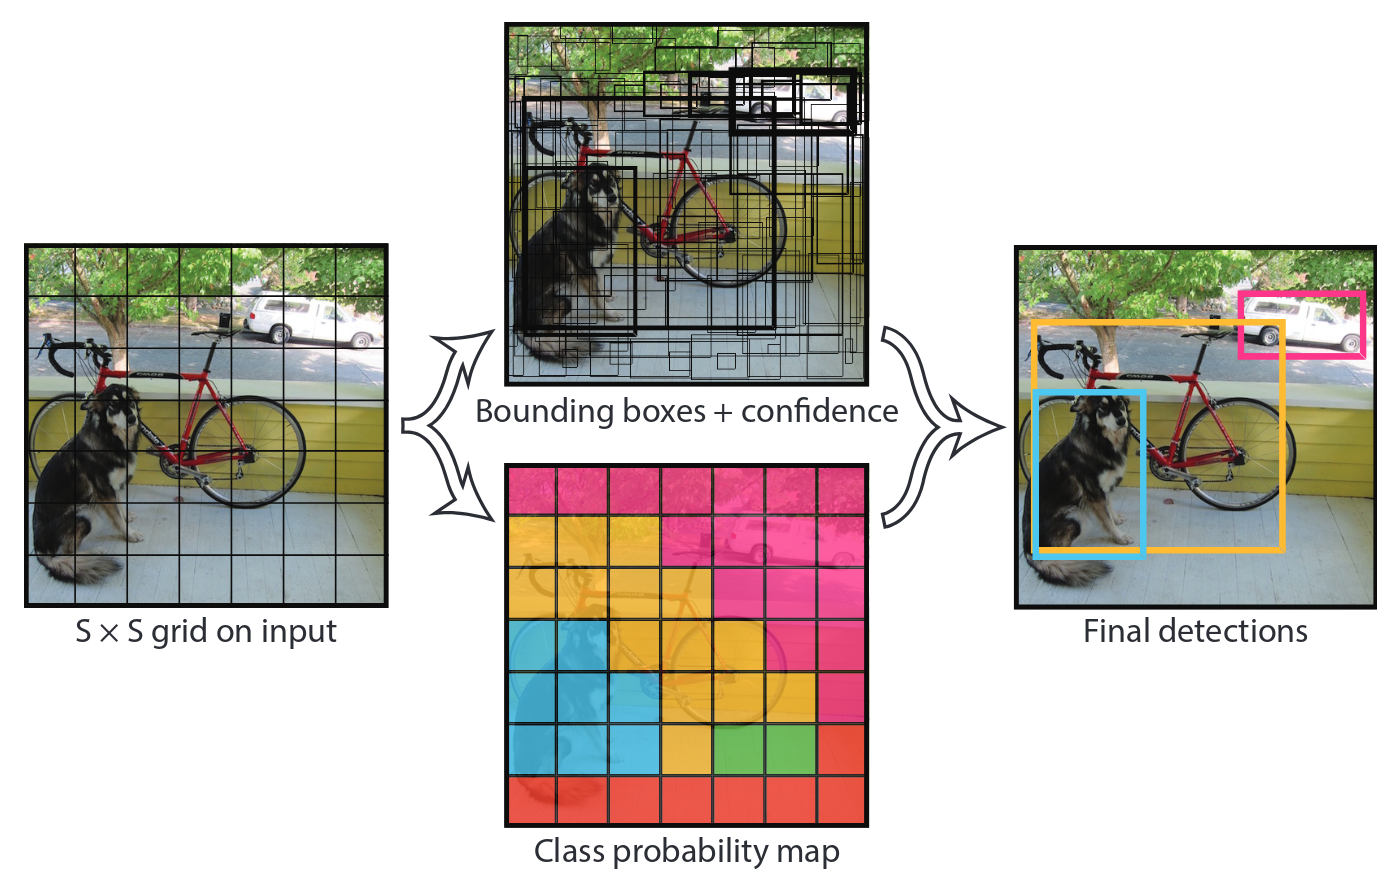
\includegraphics[width=\textwidth]{img/yoloDet}
    \caption{Detection process of \textit{YOLO}. From \cite[fig. 2]{bib:yolo}.}
    \label{fig:yoloDet} 
\end{figure}


\subsubsection{Architecture} 
\textit{YOLO} is designed as a single network that takes the input image and outputs bbox and class predictions. Design of the network is inspired by \textit{Inception} classification network. Although it does not use inception modules, it relies on the 1\x1 reduction layers to speed up 3\x3 convolutions. I\textit{YOLO} t uses 24 convolutional layers followed by two fully connected layers. Full architecture is shown on \cref{fig:yolo}. 

Multiple other versions and modifications are possible. A smaller and faster version is called \textit{Fast YOLO}. It has a similar architecture but uses only 9 convolutional layers. Another possibility to improve \textit{YOLO} is to replace the custom architecture with a more common feature extractor from a classification network. \textit{YOLO} build on top of a \textit{VGG-16} achieves better precision at the cost of half of the frames per second.

\begin{figure}
    \centering
    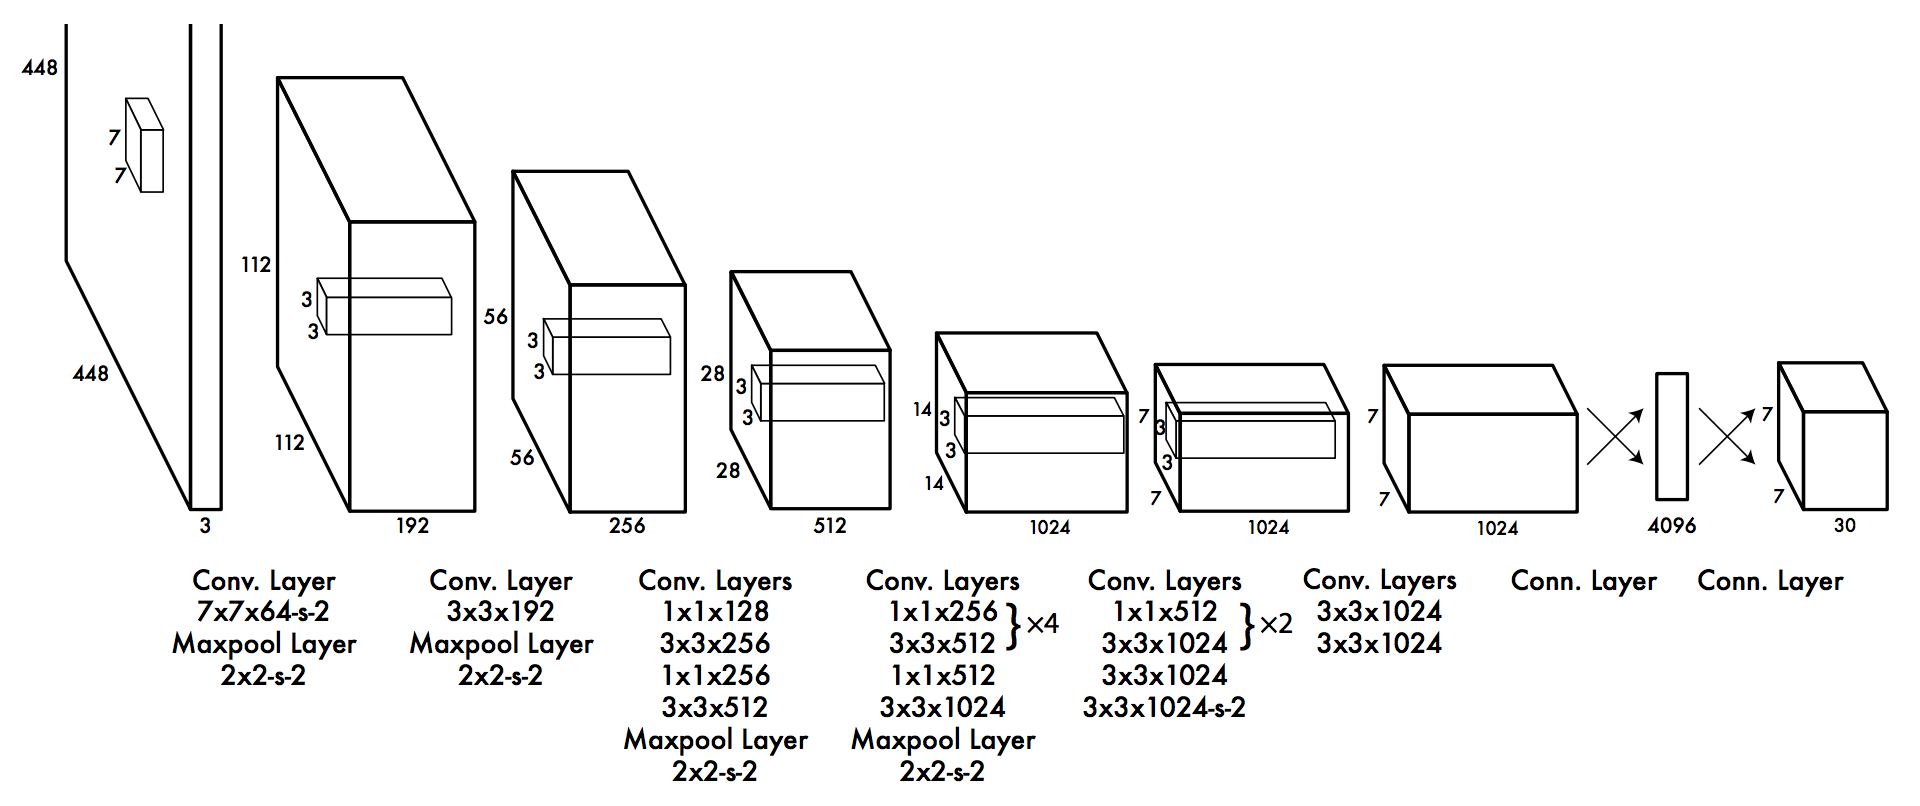
\includegraphics[width=\textwidth]{img/yoylo}
    \caption{\textit{YOLO} architecture for evaluating \textit{PASCAL VOC}. It uses 7 by 7 grid with 2 bboxes per cell. Detecting 20 categories, the output's shape is 7\x7\x30. From \cite[fig. 3]{bib:yolo}.}
    \label{fig:yolo} 
\end{figure}

\subsubsection{Training}
Although the network can be trained end-to-end, it is common for CNN to pre-train on \textit{ImageNet} dataset. This is also the case for \textit{YOLO}. First, convolutional layers are pre-trained on the \textit{ImageNet} dataset, then the detection layers are added, and the whole network is trained for detection. The model is optimized using the sum-squared error between predictions and ground-truths. The loss function is a sum of three parts, classification loss, localization loss, and bbox confidence loss. 

\paragraph{Classification loss}
\begin{align*}
\mathbf{L_{cls}} = \sum_{i=0}^{S^2}\mathbbm{1}_i^{\text{obj}} \sum_{c\in \text{class}} (p_i(c) - \hat{p}_i(c))^2
\end{align*}

\paragraph{Localization loss}
\begin{align*}
\mathbf{L_{loc}} &= \lambda_{\text{coord}} \sum_{i=0}^{S^2} \sum_{j=0}^B \mathbbm{1}_{ij}^{\text{obj}} \left[(x_i - \hat{x}_i)^2 + (y_i - \hat{y}_i)^2\right] \\
 &+  \lambda_{\text{coord}} \sum_{i=0}^{S^2} \sum_{j=0}^B \mathbbm{1}_{ij}^{\text{obj}} \left[(\sqrt{w_i} - \sqrt{\hat{w}_i})^2 + (\sqrt{h_i} - \sqrt{\hat{h}_i)^2}\right]
\end{align*}

\paragraph{Confidence loss}
\begin{align*}
\mathbf{L_{cnf}} &= \sum_{i=0}^{S^2} \sum_{j=0}^B \mathbbm{1}_{ij}^{\text{obj}} (C_i - \hat{C}_i)^2 
+ \lambda_{\text{noobj}} \sum_{i=0}^{S^2} \sum_{j=0}^B \mathbbm{1}_{ij}^{\text{noobj}} (C_i - \hat{C}_i)^2
\end{align*}

\noindent where $\mathbbm{1}^{\text{obj}}_i$ denotes if object appears in cell $i$ and $\mathbbm{1}^{\text{obj}}_{ij}$ denotes that the $j$th bounding box predictor in cell $i$ is responsible for that prediction.

The gradient of cells that do contain the object can be overpowered with the cells that do not.  Therefore, the loss from negative confidence predictions is decreased by $\lambda_{\text{noobj}} = 0.5$. And to emphasize the bbox predictions, localization loss is increased using $\lambda_{\text{coord}} = 5$.In the localization loss, we can see that the center coordinates are handled differently to width and height. The square root of width and height is used to equalize the impact of the absolute value of error in small and large boxes.


\subsubsection{Properties}
A primary virtue of \textit{YOLO} is its speed for real-time applications, and its simple architecture allows for easy training and end-to-end optimization. \textit{YOLO}'s detection layer is provided with context from the whole image which leads to less false detections than in region proposal methods. 

On the other hand, a significant problem with \textit{YOLO}'s grid-based detection system, is a limitation to one class per cell. This limitation results in the inability to detect multiple objects in close proximity, such as people in the crowd. 

\textit{YOLO} also suffers from multiple problems with precise localization. It learns to detect arbitrary shapes, which can be hard to generalize to objects in new and unusual aspect ratios. Also, it predicts the bboxes on the heavily down-sampled image which leads to further imprecision. 

\subsubsection{YOLO v2 (2017)}
\citeauthor{bib:yolo9000} \cite{bib:yolo9000}
The second version of \textit{YOLO} architecture implements a series of improvements to the original network. Compared to original 45fps on 448\x448 image, \textit{v2} achieves 59fps on 480\x480 images.


\subsection{SSD: Single Shot MultiBox Detector (2016)}
\label{sec:ssd}
\textit{SSD} is another real-time detector, aiming to outperform \textit{Faster R-CNN} by using a single network with one time evaluation. \citeauthor{bib:ssd} \cite{bib:ssd} presented this model just months after \textit{YOLO}. Even thought these networks are build on similar principles, there are multiple key differences. \textit{SSD} manages to outperform \textit{Faster R-CNN} and \textit{YOLO} both in speed and precision.

\subsubsection{Detection}
One of the main features of \textit{SSD} is that the detector network is fully convolutional and does not utilize any fully connected layers. Predictions are therefore generated for every position of a convolutional window. \textit{SSD} adopts similar concept to \textit{Faster R-CNN's} anchor boxes, this time called \textit{default} or \textit{prior} boxes. For each position of the feature map, multiple prior boxes with different aspect ratios are proposed. By default, 6 boxes are used. Contrary to \textit{YOLO}, both bbox and classification predictions are made for each position and each prior box.

Bboxes are predicted relative to prior box location which are themselves relative to feature map location. There is no bbox or region confidence value. Instead, \textit{SSD} uses an additional background class in classification predictions. Considering \textit{B} prior boxes and \textit{C} classes, \textit{SSD} generates $m\times n\times B\times (C+5)$ parameters on feature map of m\x n size.

\textit{SSD} detects objects on multiple feature maps at different scales, to accommodate detection of different sized objects. Moreover, this allows detectors on each level to focus on predicting a smaller range of bbox sizes. For the illustration of this process see \cref{fig:ssddet}.

\begin{figure}
    \centering
    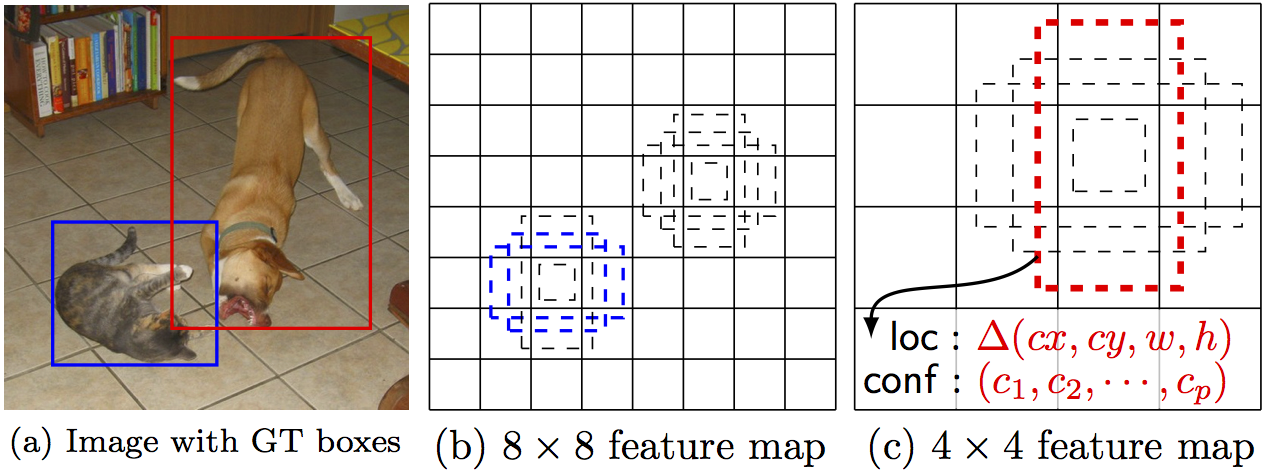
\includegraphics[width=\textwidth]{img/ssddet}
    \caption{SSD detection. (a) Input image with ground-truth boxes. (b) and (c) Predictions based on prior boxes on multiple scales of feature maps.}
    \label{fig:ssddet}
\end{figure}

\subsubsection{Architecture}
The \textit{SSD} architecture can be described as a set of three modules. A base network, extra convolutional layers and detection layers.

\begin{itemize}
    \item \textbf{Base network}'s task is to take the input image and produce a feature map. To this end, a feature extractor build from classification network is an ideal candidate. \textit{SSDs} base is build from \textit{VGG-16} network with some modifications. First of all, all fully connected layers are removed and replaced with another pair of convolution layers. \textit{Pool5} layer is also changed from 2\x2/2 to 3\x3/1 pooling. Technically, \textit{SSD} does not force any constraints on the base network, and any CNN can replace the \textit{VGG}.
    \item \textbf{Extra layers} serve the purpose of providing more feature maps on decreasing scale to the detector. Smaller feature maps aggregate more information to a smaller area and allow for detection of larger objects with small convolutional window. On the other hand, information about small objects can be lost. Therefore the use of gradually decreasing series of feature maps. \textit{Extra layers} are implemented as a sequence of convolution layers connected to the end of the \textit{base}.
    \item \textbf{Detection layers} are the final layers of the network. There is a pair of classification and localization convolutions for each feature map. Considering \textit{SSD300}, where 300 stands for the width and height of input image. Detection is performed on 6 feature maps of sizes [38, 19, 10, 5, 3, 1], using [4, 6, 6, 6, 4, 4] prior boxes respectively, producing 8732 predictions per class. First, two of those feature maps are pulled from the \textit{VGG} network, and the \textit{extra layers} provide the rest. All detection layers are implemented using 3\x3 convolutions with an appropriate number of filters, as seen on \cref{fig:VGGSSD}.
\end{itemize}

\begin{figure}
    \VGGSSD
    \caption{SSD architecture based on modified \textit{VGG-16} network. \textit{VGGs} three fully connected layers are replaced with two new convolutional layers and \textit{Pool5} layer is changed from 2\x2/2 to 3\x3/1 pooling. Detection on the first and last two feature maps uses 4 prior boxes, while the rest uses 6 boxes. See more details on \textit{VGG} in \cref{sec:VGG}.}
    \label{fig:VGGSSD}
\end{figure}


\subsubsection{Training}
\textit{SSD} pre-trains the \textit{base network} on \textit{ImageNet} dataset, and after that removes the classification layers and replaces them with \textit{extra} and \textit{detection} layers. The model is than trained for detection end-to-end. \textit{SSD} utilizes \textit{smooth L1} loss for localization and \textit{cross-entropy} loss for classification. The final loss is the sum of those two components.

Before the training, we need to figure out which prior boxes match the ground-truth annotations. For each ground-truth box, two criteria are used: a prior box with highest IoU is selected, and then, the ground-truth box is also matched to all prior-boxes with IoU higher than a threshold (0.5). Let the $x_{ij}^p = {0,1}$ be an indicator that $i$th prior box matches $j$th ground-truth box with class $p$.

To keep the balance between positive and negative samples, \textit{hard negative mining} algorithm is employed. Only top negative samples, with the highest confidence score, are chosen. The goal is to keep the ratio of positives and negatives below 1:3.

\paragraph{Localization loss} expresses the error between predicted boxes $(l)$ and ground-truths $(g)$. Predictions are generated in respect to corresponding prior boxes. Therefore, after matching the boxes, a ground-truths also need to be represented in respect to prior box $(d)$, with center $(c_x,c_y)$ and width $(w)$ and height $(h)$.

\begin{align*}
\mathbf{L_{\text{loc}}}(x,l,g) = \sum_{i\in Pos}^N \sum_{m\in(c_x, c_y, w, h)} &x_{ij}^k\text{smooth}_{L1}(l_i^m-\hat{g}_j^m) \\
\hat{g}_j^{c_x} = (g_j^{c_x} - d_i^{c_x}) / d_i^{w} \qquad& \hat{g}_j^{c_y} = (g_j^{c_y} - d_i^{c_y}) / d_i^{h} \\
\hat{g}_j^{w} = log(\frac{g_j^{w}}{d_i^w}) \qquad& \hat{g}_j^{h} = log(\frac{g_j^{h}}{d_i^h})
\end{align*}

\paragraph{Confidence loss} or classification loss, is the softmax loss over class confidences $(c)$.
\begin{align*}
\mathbf{L_{\text{cls}}}(x,c) = -\sum_{i\in Pos}^N x_{ij}^p log(\hat{c}_i^p) - \sum_{i \in Neg} log(\hat{c}_i^0) \quad\text{where} \quad\hat{c}_i^p = \frac{exp(c_i^p)}{\sum_p exp(c_i^p)}
\end{align*}

\noindent The final loss is then a weighted sum of both losses. The weight parameter $\alpha$ is set to 1. The loss is also divided by the number of matched prior boxes to keep it independent of the number of objects.

\begin{align*}
\mathbf{L}(x,c,l,g) = \frac{1}{N}(\mathbf{L_{\text{cls}}}(x,c) + \alpha\mathbf{L_{\text{loc}}}(x,l,g))
\end{align*}




% \subsection{200fps}
% \todo{ https://arxiv.org/pdf/1805.06361.pdf}

% \section{video smthing}
% \subsection{Optimizing Video Object Detection via a Scale-Time Lattice}

\section{Detection with temporal information}
In this section, we present two recent models designed specifically for detecting objects in the video. Video can provide more information to the detector, compared to a set of single independent frames, thanks to the addition of temporal information. Theoretically, using multiple consecutive video frames can provide a large improvement with dealing with detector instability, and occlusions. 

A time-space series of detected bounding boxes is usually referred to as a tube or a tublet. If such a series is generated at once for every object, it can provide smooth tracking and reduce the need for post-processing matching of detections. We use the term chunk to refer to a series of consecutive video frames, to differentiate from the batch of independent images.

However, adding another dimension to the detection model has a performance impact. It is also much harder to create a dataset suitable for training of detectors with a temporal dimension because a whole series of frames needs to be precisely annotated. Of course we can find a few public datasets e.g. \textit{ImageNet VID}\footnote{\url{http://image-net.org/challenges/LSVRC/2017/\#vid}}, \textit{YouTube-8M}\footnote{\url{https://research.google.com/youtube8m}} and some smaller ones like \textit{HollywoodHeads}\footnote{\url{https://www.di.ens.fr/willow/research/headdetection}}.

This section presents two approaches to adding a temporal information to a object detector. First presented method adopts the approach of region proposal methods and the second one is based on single stage detector.


\subsection{Tube-CNN (2018)}
\label{sed:tubecnn}
The architecture of this detector is very similar to \textit{Fast-RCNN} with the added temporal dimension. The main idea is based on region/tube proposals and the following classification network for those regions. \citeauthor{bib:tubeCNN} \cite{bib:tubeCNN} proved that using a temporal information provided by continuous video frames enhances a precision of the detector. On the other hand, this approach adds more complexity to slower than real-time \textit{Faster-RCNN} detector. The resulting network achieves only low single digit frame per second values, depending on configuration. 

\subsubsection{Tube proposal network}
Tube proposal generation begins with a feature extraction on a chunk of video frames. After the processing of all frames individually, feature maps are stacked together in the temporal dimension. Then, volumetric convolutional layers (conv3d) are applied to produce a feature volume.

Analogously to \textit{Faster-RCNN}, each position in this feature volume is used to create tube proposals using \textit{K} anchor tubes. The proposal for each anchor consists of the \textit{objectness} and position parameters. The \textit{objectness} score reflects the probability of the presence of the same objects as opposed to a background. 

IoU value for tubes is defined as a minimum of spatial IoU at the ends of tubes. The number of proposals is reduced by eliminating tubes with high overlap using a non-maximum suppression based on \textit{objectness} score. 

A provided data for the training usually consists of a series of ground-truth boxes for individual frames. During training of TPN, a series of ground-truth boxes is approximated by a ground-truth tube. Those tubes are then matched against the tube proposals using an IoU threshold. A tube proposal network is designed only to consider tubes corresponding to linear motion in order to limit the complexity. 

\subsubsection{Detection network}
\textit{Tube-CNN}, as the name suggests, is a fully convolutional network with the task to extract feature maps from the incoming chunk of images, and using the given tube proposals, classify the tubes and refine the object positions. 

Same as in TPN, the feature extraction is done independently on each frame using some general extractor, e.g., \textit{ResNet}. Feature maps are then stacked to form a spatio-temporal feature volume. Unfortunately, the provided research paper does not clarify whether the proposal and detection networks share the same extraction layers or not.

A Tube-of-Interest (ToI) pooling is employed on feature volume to select the sub-volume corresponding to each tube proposal. The selected volume is then max-pooled into a fixed-size feature and subsequently used as an input for a classifier. A general convolutional classifier with soft-max activation is used. 

The regression branch of the network predicts the exact position of the object in the first and last frame of the tube. Both regressions begin with a RoI pooling on the corresponding feature maps and continue with convolutional layers to produce the positional parameters. 

The detection process is illustrated in \cref{fig:tubecnn}.


\begin{figure}
    \centering
    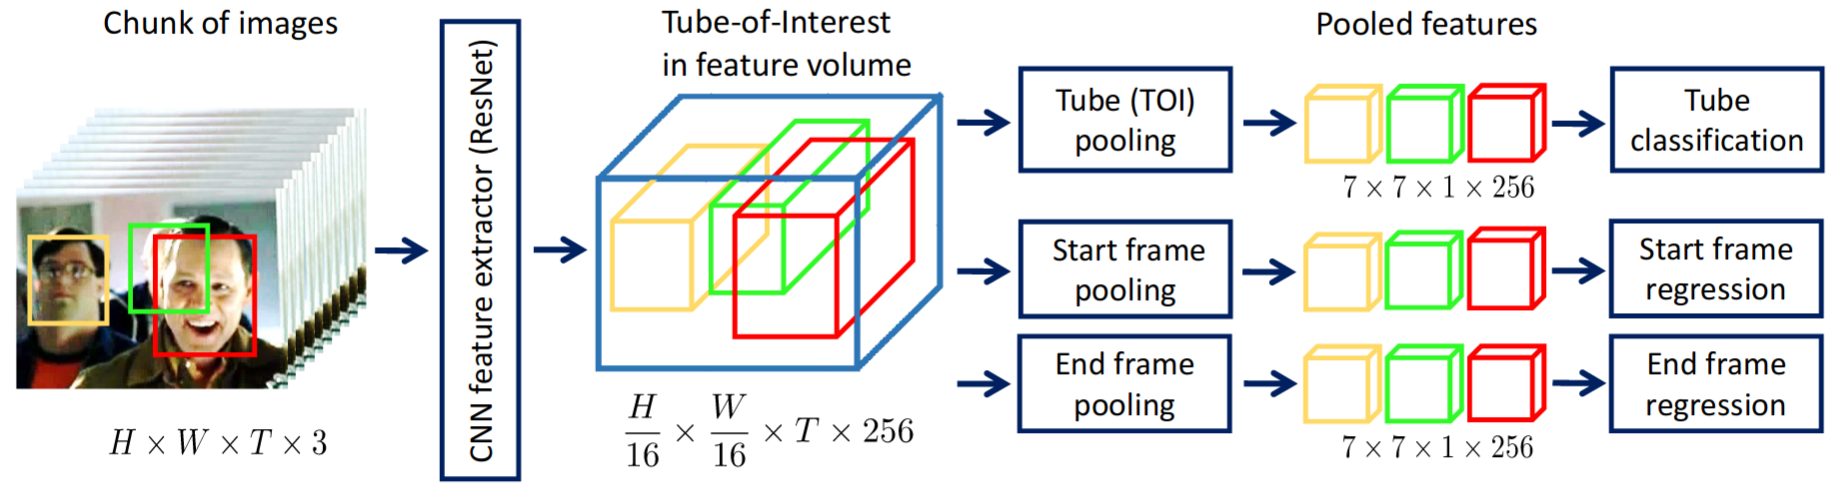
\includegraphics[width=\textwidth]{img/tubecnn}
    \caption{Architecture of Tube-CNN for object detection. Taken from \cite[fig.~2]{bib:tubeCNN}.}
    \label{fig:tubecnn}
\end{figure}


\subsection{TSSD (2019)}
\label{tssd}
\citeauthor{bib:tssd} combine the \textit{SSD} with recurrent networks \cite[chpt.~10]{bib:dlbook}, namely ConvLSTM cells introduced by \citeauthor{bib:convlstm} \cite{bib:convlstm}, to create a \textit{temporal single-shot detector} (TSSD) \cite{bib:tssd}. They also proposed a tracking module with \textit{Online Tubelet Analysis} working on top of the \textit{TSSD}.
Compared to \textit{SSD}'s 45fps, \textit{TSSD} achieves 27fps on \textit{ImageNet VID} dataset.  

\subsubsection{Architecture}
\textit{TSSD} is based on a standard backbone of \textit{SSD} implemented on fully convolutional \textit{VGG-16} base with extra layers (see \cref{sec:ssd}). This base provides six feature maps that are used for classification and bbox regression in \textit{SSD}. However, \textit{TSSD} applies one more layer on the feature maps before detection. This is where the temporal information comes into effect, using the aforementioned convolutional LSTM cells. Two \textit{Attentional ConvLSTM} (AC-LSTM) cells are deployed, one for the bottom three feature maps and one for the top three. Only a small adjustment has been made to the underlying VGG network, that being lowering the number of channels in the second feature map to 512, to equalize the channels in all low-level feature maps. The outputs of both cells are then used for classification and regression in the same way the \textit{SSD} would do. Details of \textit{TSSD} implementation, including details on \textit{AC-LSTM} can be seen on \cref{fig:tssd}. 

Features contributing to positive object detections are unevenly distributed in feature maps and through the scales. Authors proposed the \textit{Attentional ConvLSTM} cell with the goal of background and scale suppression.  The temporal attention module in \textit{AC-LSTM} provides the rest of the cell with object-aware features. 

\begin{figure}
    \centering
    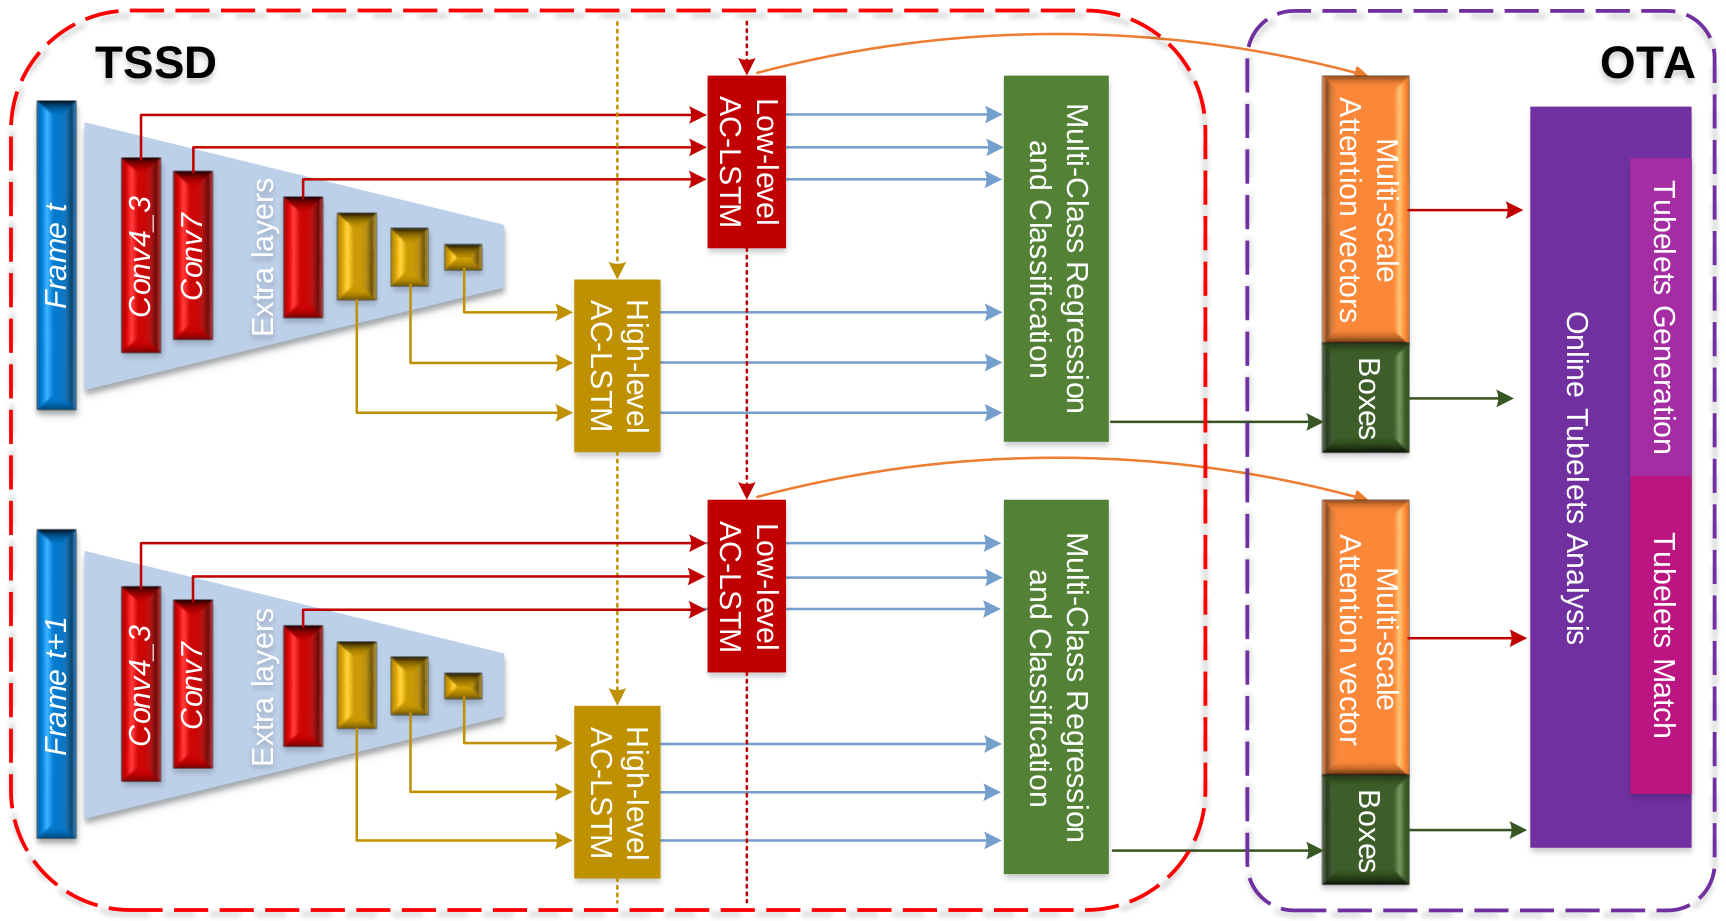
\includegraphics[width=\textwidth]{img/tssd}
    \caption{Architecture of \textit{TSSD} (left) and \textit{AC-LSTM} cell (right). \textit{c} denotes concatenation; \textit{Chw-x}, \textit{Elw-x} represent channel-wise and element-wise multiplication, respectively; \textit{+} is element-wise summation. From \cite[fig.~2,~3]{bib:tssd}.}
    \label{fig:tssd}
\end{figure}


\subsubsection{Training}
Similarly to \textit{SSD}, the loss function of \textit{TSSD} has multiple objectives weighted by $\alpha, \beta, \gamma$ and $\xi$ constants.

\begin{align*}
\mathbf{L} = \frac{1}{N}(\alpha\mathbf{L_{\text{loc}}} + \beta\mathbf{L_{\text{cls}}}) + \gamma\mathbf{L_{\text{att}}} + \xi\mathbf{L_{\text{asc}}}
\end{align*}


Where $\mathbf{L_{\text{cls}}}$ and $\mathbf{L_{\text{loc}}}$ are defined according to \textit{SSD} (\cref{sec:ssd}) and \textit{N} is the number of matched boxes.

Attention loss is calculated as a binary cross-entropy loss between ground-truth attention map $A_g$ and prediction maps $A_{_{sc}}$ for each scale $sc$. $A_g$ is a binary map with ones on positions inside ground-truth boxes. Each predicted attention map is up-scaled ($A^{up}_{p_{sc}}$) to match the dimensions of the $A_g$.

\begin{align*}
\mathbf{L_{\text{att}}} = \sum_{sc=1}^6 \mu (-A^{up}_{p_{sc}} log(A_g) - (1-A^{up}_{p_{sc}})log(1-A_g))
\end{align*}

Video frames are generally temporally consistent. Therefore we also expect consistency in detections on short sequences of frames. We can suppress fluctuations in temporal detections by defining association loss. We use class-discriminative score list ($sl$) to represent detection in a frame. $sl$ sums up top-k predictions after application of NMS.

\begin{align*}
\mathbf{L_{\text{asc}}} = (\sum_{t=1}^{seq} sl_t - sl_{avg})/seq
\end{align*}

Where $sl_t$ denotes the score list in frame $t$, $sl_avg$ denotes the average list in a sequence and $seq$ represents the sequence length. 
